
\chapter{Functions (2 of 2)}

Like many things in life, writing functions is best learned by example. This
chapter will feature more of them that you can learn from and imitate.

\subsubsection{Basketball scoring: \texttt{bb\_pts()}}

Continuing the sports theme, the total points a basketball player scores is
related to the number of shots she makes of various kinds. Typically, the ``box
score'' of a game (see example in Figure~\ref{boxScore}) reports three scoring
stats: (1) the \textit{total} number of ``field goals''\footnote{A ``field
goal'' in basketball just means ``a regular basket'' -- \textit{i.e.}, not a
free throw penalty shot.} a player made and attempted, (2) the number of these
field goals, if any, that were for three points\footnote{In most leagues, a
basket is worth 2 points unless the shooter was farther than a certain distance
from the hoop when she shot it, in which case it's worth 3.}, and (3) the
number of free throws (``easy'' penalty shots) the player attempted and made.

Confusingly, (1) \textit{includes} (2). In other words, if the first number is
4 and the second is 1, the player didn't score 4 regular two-point baskets and
1 three-pointer, but rather \textit{3} two-point baskets and 1 three-pointer.

\begin{figure}[ht]
\centering
\fbox{
\mbox{
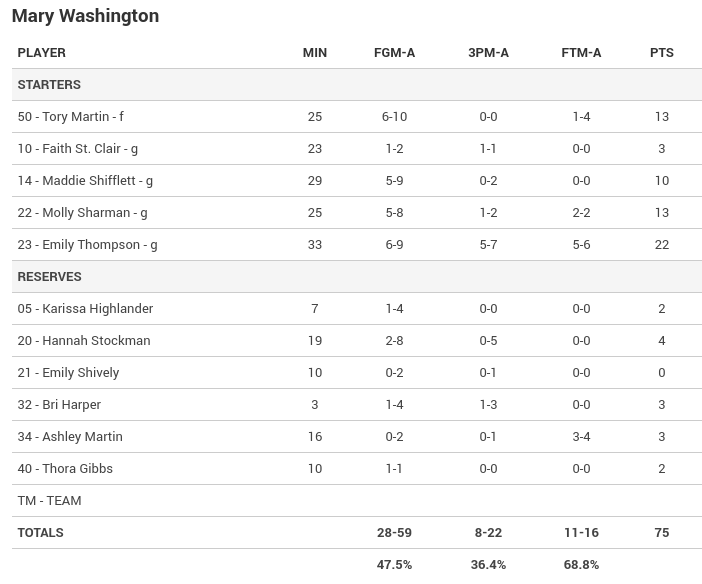
\includegraphics[width=0.8\textwidth]{boxScore.png}
}
}
\medskip
\caption{A basketball box score.}
\label{boxScore}
\end{figure}

In Figure~\ref{boxScore}, the \textsf{FGM-A} column gives the first of these
three categories, \textsf{3PM-A} the second, and \textsf{FTM-A} the third. The
\textsf{PTS} column gives the total number of points that player scored. (For
example, Molly Sharman made 5 of her 8 attempted field goals, one of which was
for three points, and she also converted both free throw attempts.)

All that took a lot longer to explain than the corresponding Python function:

\index{bb\_pts@\texttt{bb\_pts()}}

\begin{Verbatim}[fontsize=\small,samepage=true,frame=single,framesep=3mm]
def bb_pts(fgm, threep_fgm, ftm):
    return ((fgm - threep_fgm) * 2) + (threep_fgm * 3) + (ftm * 1)

torys_pts = bb_pts(6, 0, 1)
print("Tory scored {} points.".format(torys_pts))
print("Emily scored {} points.".format(bb_pts(6, 5, 5)))
print("The Lady Eagles scored {} points!".format(bb_pts(28, 8, 11)))
\end{Verbatim}
\vspace{-.2in}

\begin{Verbatim}[fontsize=\small,samepage=true,frame=leftline,framesep=5mm,framerule=1mm]
Tory scored 13 points.
Emily scored 22 points.
The Lady Eagles scored 75 points!
\end{Verbatim}

\index{PEMDAS}

Strictly speaking you don't need all those bananas (regular PEMDAS
order-of-operations applies) but I think it's a good idea to include them for
clarity and grouping.

\subsubsection{``Exceptions'': \texttt{mean\_no\_outliers()} and \texttt{quiz\_avg()}}

Sometimes we want to take the straight average of a data set, but other times
we may want to filter out any strange or exceptional cases. Let's say we're
computing the average age of a classroom of college students, but we want to
remove any adult learners over 30 since that would skew the result. We could do
this sort of thing with a function like this:

\index{mean\_no\_outliers@\texttt{mean\_no\_outliers()}}
\index{low\_cutoff@\texttt{low\_cutoff}}
\index{high\_cutoff@\texttt{high\_cutoff}}

\begin{Verbatim}[fontsize=\small,samepage=true,frame=single,framesep=3mm]
def mean_no_outliers(data, low_cutoff, high_cutoff):
    return data[(data >= low_cutoff) & (data <= high_cutoff)].mean()

our_class = np.array([20,18,19,18,22,21,76,20,22,22,21,18])
print("The average age (excluding outliers) is {}.".format(
    mean_no_outliers(our_class, 0, 30)))
\end{Verbatim}

\vspace{-.2in}

\begin{Verbatim}[fontsize=\small,samepage=true,frame=leftline,framesep=5mm,framerule=1mm]
The average age (excluding outliers) is 20.09090909090909.
\end{Verbatim}

We've provided two arguments to the function besides the data set itself: a
lower and upper bound. Anything falling outside that range will be filtered
out. In the example function call, we passed 0 for the \texttt{low\_cutoff}
since we didn't desire to filter anything at the low end. (If we wanted to,
say, also remove children from the data set, we could have set that to 16 or
so.)

By the way, you might find the number of decimal places printed to be
unsightly. If so, we could enhance our function by rounding the result to (say)
two decimals with NumPy's \texttt{round()} function:

\index{round@\texttt{round()} function (NumPy)}

\begin{Verbatim}[fontsize=\footnotesize,samepage=true,frame=single,framesep=3mm]
def mean_no_outliers(data, low_cutoff, high_cutoff):
    return np.round(data[(data >= low_cutoff) & (data <= high_cutoff)].mean(),2)

print("The average age (excluding outliers) is {}.".format(
    mean_no_outliers(our_class, 0, 30)))
\end{Verbatim}
\vspace{-.2in}

\begin{Verbatim}[fontsize=\small,samepage=true,frame=leftline,framesep=5mm,framerule=1mm]
The average age (excluding outliers) is 20.09.
\end{Verbatim}

At this point you might think this function is getting pretty big for a
one-liner. I agree. Let's split it up and use some temporary variables to make
it more readable:

\begin{Verbatim}[fontsize=\small,samepage=true,frame=single,framesep=3mm]
def mean_no_outliers(data, low_cutoff, high_cutoff):
    filtered_data = data[(data >= low_cutoff) & (data <= high_cutoff)]
    filtered_average = np.round(filtered_data)
    return np.round(filtered_average,2)
\end{Verbatim}

Much clearer!

\medskip

A related but different example would be to remove a fixed \textit{number} of
data points from the end, instead of data points outside a specified range. For
instance, in my classes, I often give students (say) eight quizzes during a
semester, and drop the lowest two scores. That could be done with:

\index{sorting@sorting (arrays)}
\index{sort@\texttt{np.sort()} (NumPy)}
\index{quiz\_avg@\texttt{quiz\_avg()}}
\index{Filbert}

\begin{Verbatim}[fontsize=\small,samepage=true,frame=single,framesep=3mm]
def quiz_avg(quizzes):
    dropped_lowest_two = np.sort(quizzes)[2:len(quizzes)]
    return dropped_lowest_two.mean()

filberts_quizzes = np.array([7,9,10,7,0,8,4,10])
print("Filbert's avg score was {}.".format(quiz_avg(filberts_quizzes)))
\end{Verbatim}
\vspace{-.2in}

\begin{Verbatim}[fontsize=\small,samepage=true,frame=leftline,framesep=5mm,framerule=1mm]
Filbert's avg score was 8.5.
\end{Verbatim}

Filbert's 0 and 4 were dropped, leaving him with a pretty good semester score.

The trick to this implementation is \textit{sorting} the quiz scores. Once you
do that, it's easy to pick out the top six to take the average, since the
lowest two scores will be at the beginning of the (sorted) array. Two notes
here:

\index{slice}
\index{boxies (square brackets)}
\index{[]@\texttt{[]} (boxies)}

\begin{compactitem}
\item We use the \texttt{np.sort()} function, not the \texttt{.sort()} method,
since we don't want to permanently change the order of \texttt{quizzes}. We
only need a temporarily sorted copy so we can omit the lowest two entries.
\item That business in the boxies (``\texttt{[2:len(quizzes)]}'') is a
\textbf{slice} (recall chapter~\ref{ch:arraysInPython1}) which says ``only give
me entries number 2 through the end of the array.'' And that's exactly what the
doctor ordered to omit the first two.
\end{compactitem}


% any_zeros()
% quiz_avg()
